\section{Introduction}
\label{sec:introduction}
Cooperative perception extends sensing horizons and resolves occlusions by aggregating complementary multi-agent observations~\cite{opv2v,v2vnet,heal}. While camera-only systems avoid expensive LiDARs, practical deployment is degraded by acute sensitivity to spatial misalignment from localization errors (e.g., GNSS multipath and latency). As contrasted across spatial alignment paradigms in Fig.~\ref{fig:pose_noise}, the underlying alignment mechanism fundamentally determines collaborative robustness.

\begin{figure}[t]
\centering
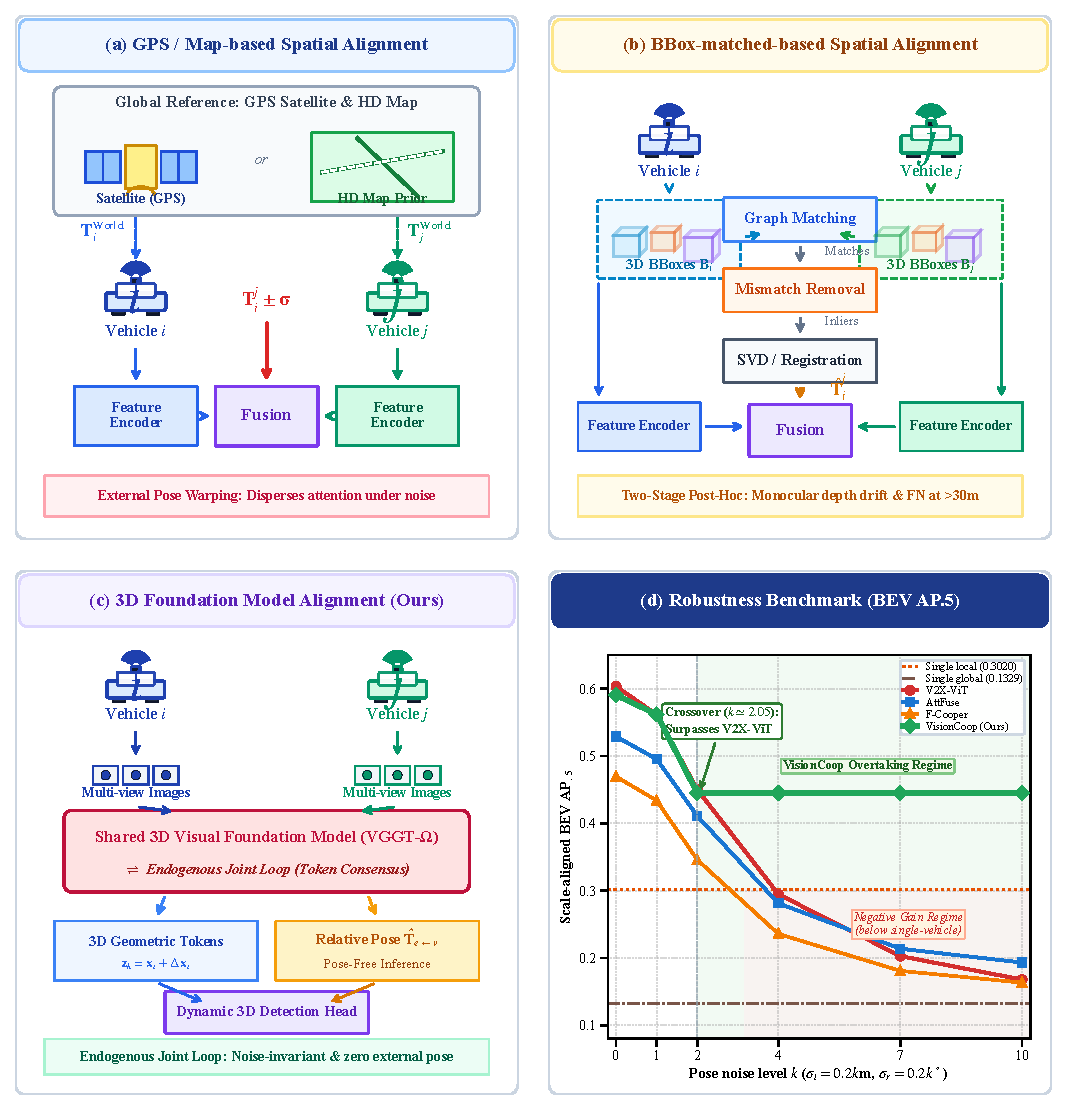
\includegraphics[width=0.96\columnwidth]{figures/teaser_stacked.pdf}
\caption{Spatial alignment paradigms and OPV2V benchmark. (a)~\emph{GPS/Map}: external-pose warping. (b)~\emph{BBox-match}: post-hoc registration. (c)~\emph{3D foundation model} (Ours): endogenous joint loop. (d)~\emph{Benchmark}: feature fusion collapses into negative gain; \method{} remains noise-invariant (44.52\% AP$_{.5}$), crossing V2X-ViT ($k \ge 2.05$).}
\label{fig:pose_noise}
\end{figure}

Existing spatial alignment paradigms face intrinsic limitations: \emph{feature-level fusion}~\cite{v2xvit,opv2v,fcooper} (Fig.~\ref{fig:pose_noise}(a)) warps bird's-eye-view (BEV) features using noisy external poses, dispersing cross-attention and collapsing into negative collaborative gain under noise (Fig.~\ref{fig:pose_noise}(d)); conversely, \emph{two-stage box registration}~\cite{v2xreg,freealign} (Fig.~\ref{fig:pose_noise}(b)) matches bounding boxes post-hoc, but is strictly bounded by monocular depth uncertainty and false negatives at long ranges ($>30$\,m).

Recently, 3D visual foundation models~\cite{dust3r,vggt,omega} provide a promising alternative (Fig.~\ref{fig:pose_noise}(c)). Pre-trained on diverse multi-view imagery, models such as VGGT-$\Omega$ internalize 3D geometry and dense surface depth, providing a foundation for cooperation without external poses. However, applying them to cooperative perception exposes a fundamental \emph{reconstruction-to-detection gap}: foundation models natively target low-level surface reconstruction rather than oriented 3D boxes. Adapting foundation representations encounters three primary obstacles: (1)~\emph{Surface-to-Center Disparity:} Features capture visible surfaces rather than unobserved 3D centroids. (2)~\emph{Scalar Depth Ambiguity:} Raw scalar depth lacks an oriented 3D frame, perturbing query attention (Sec.~\ref{sec:ablation}). (3)~\emph{Dense Representation Overhead:} Projecting features into dense BEV grids or pseudo-point clouds~\cite{pointpillars} incurs substantial latency overhead (Fig.~\ref{fig:runtime}) while re-imposing coordinate dependencies.

To address these challenges, we propose \textbf{\method{}}, directly coupling a shared 3D visual foundation model to cooperative 3D detection. Rather than rasterizing features into rigid global grids, \emph{Surface-Guided Query Initialization} lifts surface tokens into 3D space and aggregates learned offset votes toward latent object centroids, seeding queries with physical priors. Subsequently, \emph{Depth-Guided Iterative Query Refinement} establishes an active geometric verification loop: evolving 3D box hypotheses serve as adaptive local frames, where an 8D rotation- and scale-normalized descriptor measures offsets between box boundaries and physical surfaces, translating ambiguous depth into structured geometric feedback. By confining query updates to local coordinates and utilizing backbone token exchange to infer relative vehicle poses $\hat{T}_{e \leftarrow v}$, \method{} unifies semantic refinement with global spatial consensus without external poses at inference.

Our contributions are threefold. First, we integrate 3D visual foundation models into cooperative perception without consuming external poses at inference, characterizing robustness under pose noise. Second, we analyze scalar depth integration failures and formulate depth-guided iterative query refinement, achieving \textbf{+7.31} points in $\text{AP}_{.5}$ over direct query without depth and outperforming naive scalar concatenation by \textbf{+19.68} points (Sec.~\ref{sec:ablation}). Third, on OPV2V, \method{} maintains 44.52\% scale-aligned AP$_{.5}$ across the noise grid, crossing V2X-ViT between $k=2$ and $k=4$ with 0.55$\times$ normalized inference cost over pseudo-point-clouds; on DAIR-V2X, cross-domain fine-tuning reaches \textbf{0.706\,m} translation and \textbf{0.428$^\circ$} rotation errors.

\begin{figure*}[t]
\centering
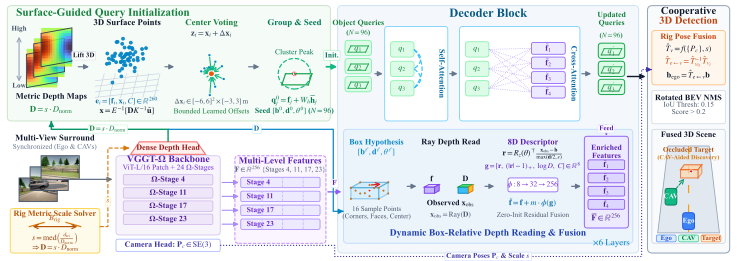
\includegraphics[width=0.95\textwidth]{figures/architecture(1).svg}
\caption{\method\ overview: a shared VGGT-$\Omega$ backbone couples camera, depth, and query-detection branches under known within-vehicle calibration.}
\label{fig:architecture}
\end{figure*}
